% !TEX root = arbeit.tex
\section{Setup}\label{sec:setup}

	% Noch Kapitelreferenz rausnehmen, da dass jetz in einem Kapitel zusammengefasst ist.
	This chapter includes the stand of the NIM prototype as it was in January 2018 (Chap. \ref{subsubsec:setupProto}). During test campaigns (Chap. bla) some parts such as the reflectron and the antechamber were exchanged and tested on the prototype. In May 2019 the tests with the NIM ProtoFlight Model (PFM) started. Chapter \ref{subsubsec:setupPFM} describes the NIM PFM as it was at the beginning of the test campaign. During the tests, improvements had to be done such as adaptations of the ion source and improvements on the detector.\\
	In Chap. \ref{subsec:setupTestTools} the test facilities are described. Tests with a neutrals particle beam were performed with the CASYMIR test facility at the University of Bern. % Ref.
	% Noch STROFIO chamber erwähnen und schreiben, welche tests man in dieser Kammer machen kann.
	% Pumpstand 2 überhaupt erwähnen? Gain Kurve mit dem einen anderen detector aufzeichnen und rein kopieren. Gibt dazu nicht viel zu schreiben.
	
	
	\begin{comment}
	The goal of this chapter is to show NIM in the current lab equipment. An 'as is' state.
	Instrument in vacuum chamber, Mechanical description. Theoretical description is in the theory part.
	Cabeling with schema for all test configurations (have a look at the TRR schema).
	IS based on the design of Abplanalp 2009 if so. Look it up for NIM.
	With which IS, reflectron, detector. Short description of the different parts as they were for the first tests. (IS, reflectron, detector type). With pictures. Short description of the IS types of the PFM (ref. to Davides paper. Give a bit a more detailed description)
	Lab electronics, cabling? Or just reference to Stefan's Diss? Used standard settings such a pulser timings, UMCP, filament emission current, chamber pressure.
	(The specified setting for each measurement will be mentioned in chapter experiments for the different settings)
	\end{comment}
	
	\subsection{NIM Sensor Models}\label{subsec:setupInst}
	In this chapter, the NIM Prototype and the design of the NIM ProtoFlight Model (PFM) are described. The Prototype was build by Stefan Meyer and he also designed the NIM PFM \cite{Diss_Meyer}. The tests in Chapter \ref{sec:Exp} start with the configuration of the instruments as they are stated in this chapter.\\
	Fig.\ref{fig:SetupProtoISSim} shows the SIMION model of the Prototype ion-source Fig.\ref{fig:SetupPFMISSim} shows the ion-source of the PFM and Fig.\ref{fig:SetupFilElSim} shows the filament housing of the Prototype (left) and of the PFM (right). The PFM has seven electrodes less then the prototype to simplify the source. Manly LV electrodes were taken together (IS 1\& 2, IS 3 \& 4, IS 6 \& 7). IS 10 was removed and IS 11 was shifted towards the ionisation region. In the filament housing the filament repeller electrodes Fil 2-5 were taken together to one single repeller electrode Fil 2. The repeller electrode was splitted in 4 to compensate the filament position in case the filament was badly adjusted. For the PFM, the mounting of the filament holder was improved, therefore these 4 electrodes could be taken together to one single electrode.\\

	% Comparison between the two designs/ types of the main structures.
	% Reflectron
	% Detector
	
	% Fig.\ref{fig:SetupProtoISSim}-\ref{fig:} show the SIMION models of the Prototype ion-source, the filament housing, the ion-mirror and the detector. Fig.\ref{fig:SetupProto} shows the NIM Prototype as it was at the beginning of the measurement campaigns. Detailed cable schema and connection to the laboratory power supplies can be found in \cite{Diss_Meyer} Chap. 4.2.

		
		\begin{comment}
		Flight electronics
		Have a look how this is actually done/ included. -> Separate Subchapter included in the PFM chapter. Paper description is sufficient. May add here the schema again for the further description for the tests how it is tested.
		Antechamber, reflectron, detector. Grober Aufbau ist bis hierhin schon erklärt. 
		
		The cabeling can be referenced to the thesis for the Prototyp.
	
		NIM Instrument description overview. Startconfiguration.
		
		Foto von Rack von Stefan reinkopieren (Fig. 4.12) damit man sieht, wie es betrieben wurde. Liste welche Elektrode wo angeschlossen wird (schauen, ob das gleich ist wie in seiner Diss. Ansonsten Referenz und nur Anpassungen einfügen)
		
		
		Schema of the Prototype with the lenses
		IS with 8 lenses and one filament holder (flight 7 lenses, 2 filament holders)
		small antechamber with edge, one entrance hole at 90° (flight 80mm diam., 2 holes at +-60° relative to normal)
		Prototype reflectron with ring electrodes (flight has 3 electrodes with a linear increasing resistance in between them)
		Pulser: lab pulser (flight still under development -> tests later)
		\end{comment}
		
		\textbf{Ion-Optical System Prototype}\\
		
		\begin{figure}[h] % Bild durch Bild mit Markierungen ersetzen
			\centering
			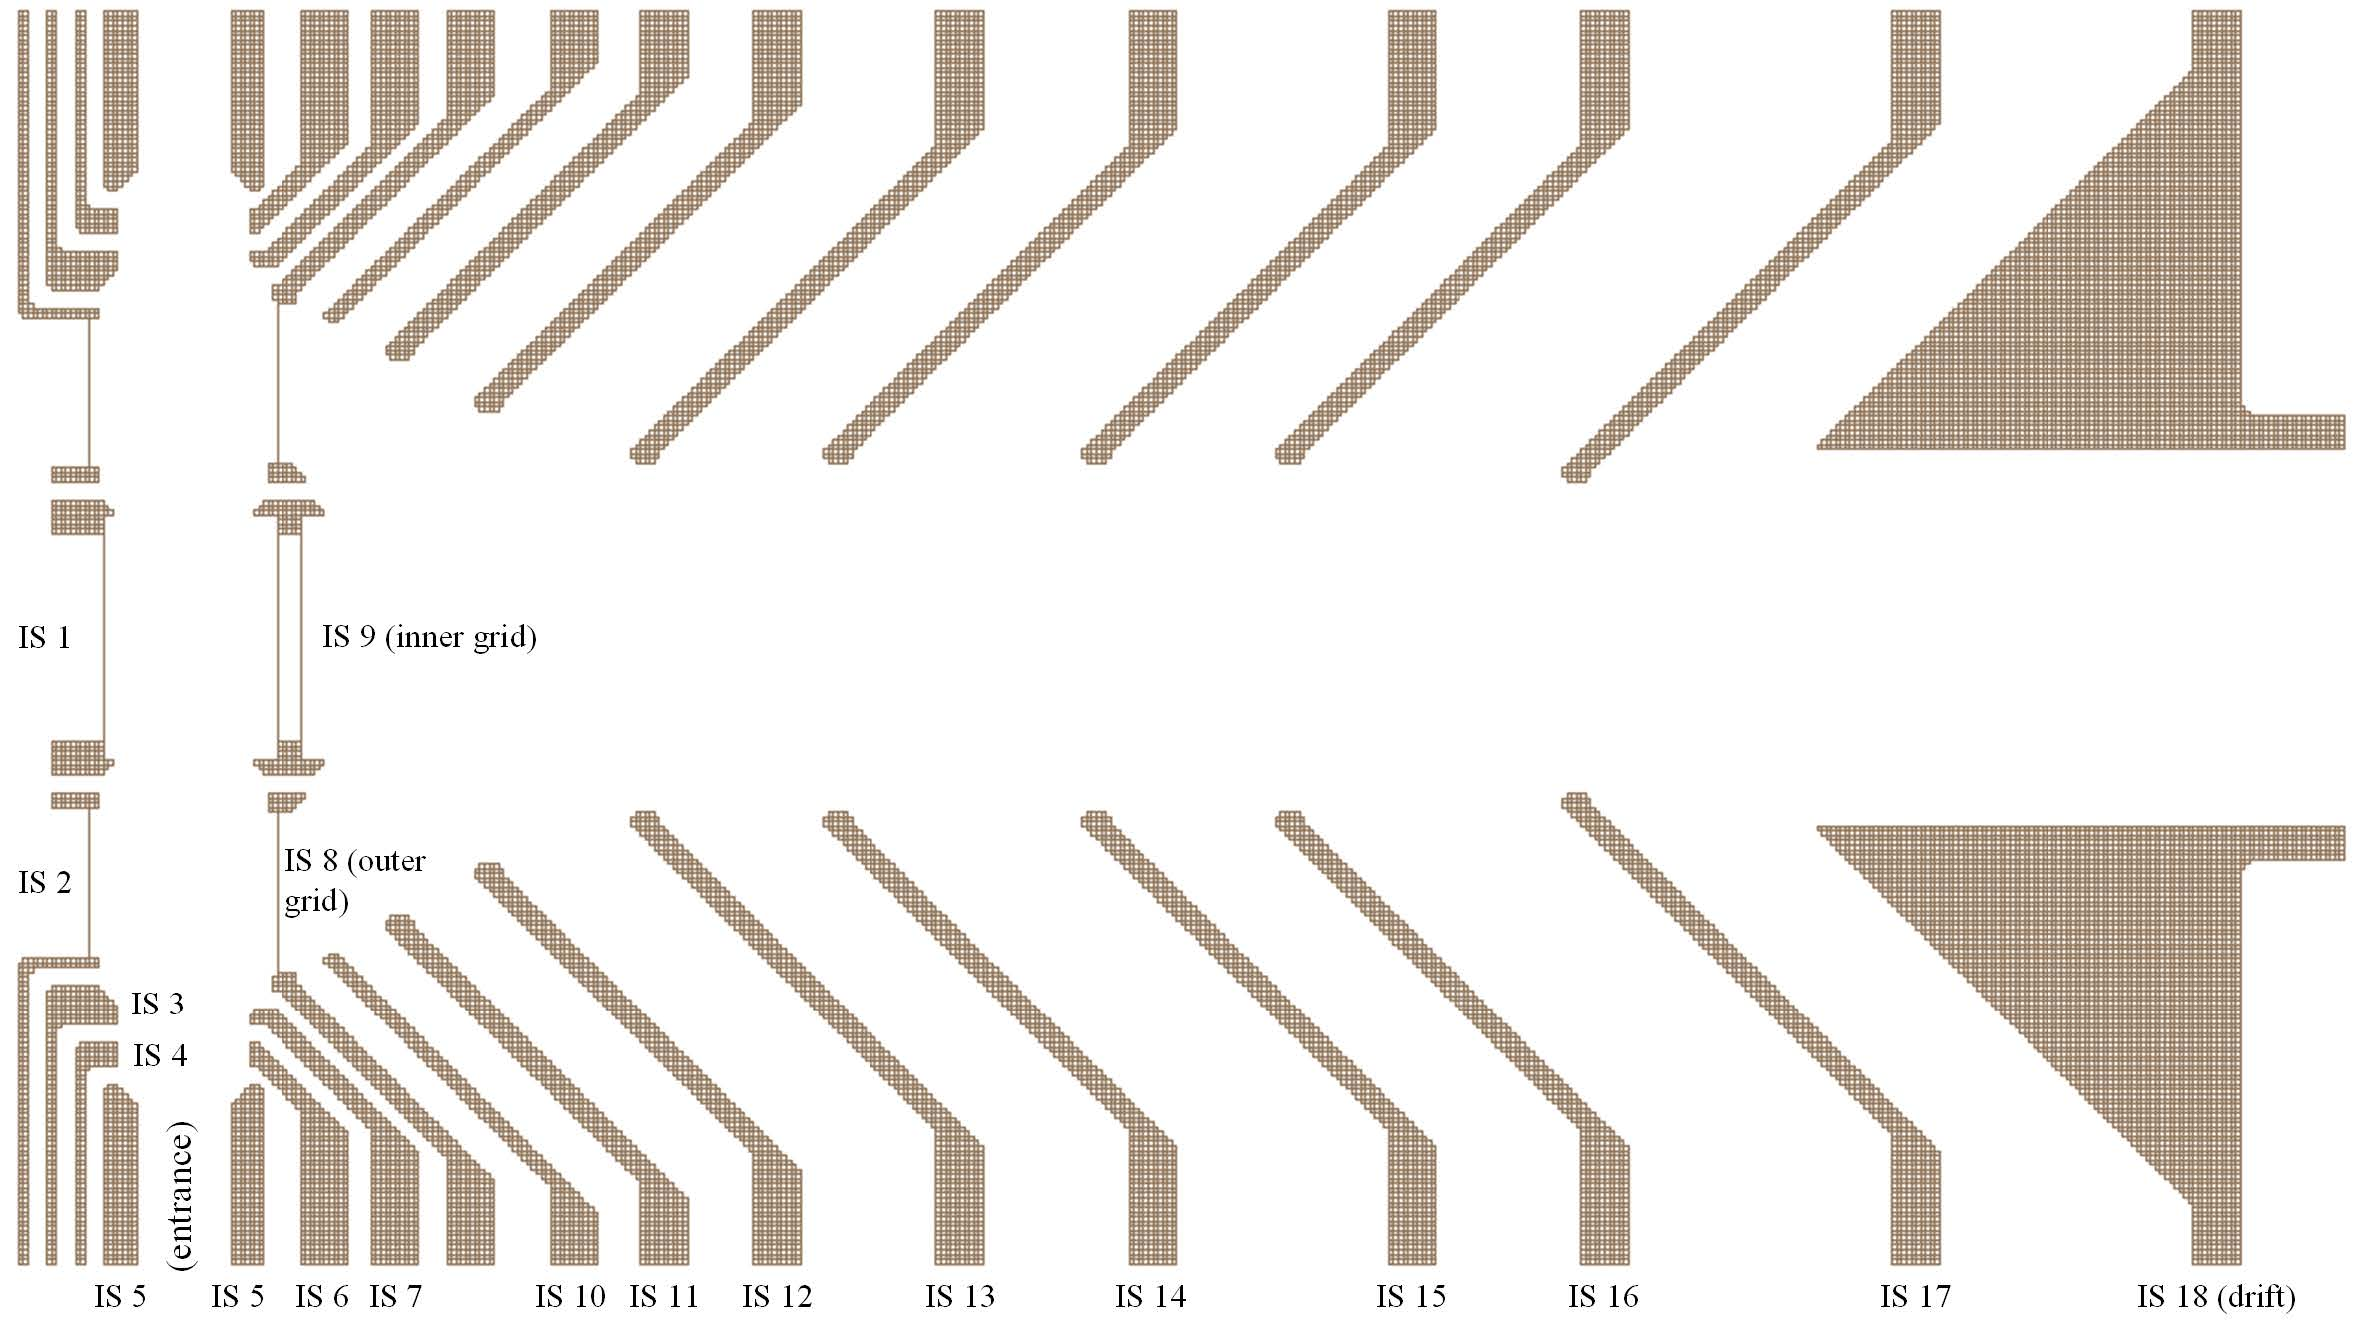
\includegraphics[width=0.9\textwidth]{Setup/Prototype_IS_sim.jpg}
			\caption{SIMION Model of the Ion-Source of the NIM Prototype \cite{Diss_Meyer}.}
			\label{fig:SetupProtoISSim}
		\end{figure}
		
		\begin{figure}[h] % Bild ersetzen. Evt noch Markierungen einfügen. IS bei den Nr. evt. noch einfügen.
			\centering
			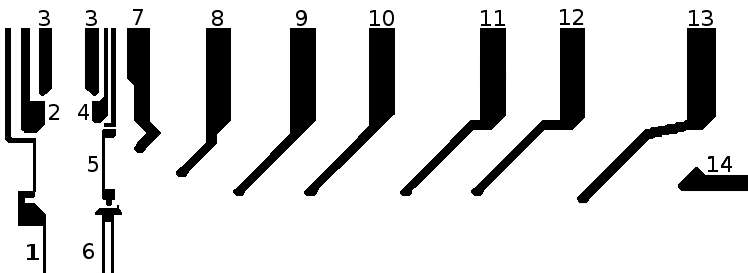
\includegraphics[width=0.9\textwidth]{Setup/PFM_IS_sim.png}
			\caption{SIMION Model of the Ion-Source of the NIM ProtoFlight Model.}
			\label{fig:SetupPFMISSim}
		\end{figure}
	
		\begin{figure}[h] % In Bild noch Fil 7/ Fil 4 durch IS5/ IS3 ersetzen.
			\begin{subfigure}{0.5\textwidth}
				\centering
				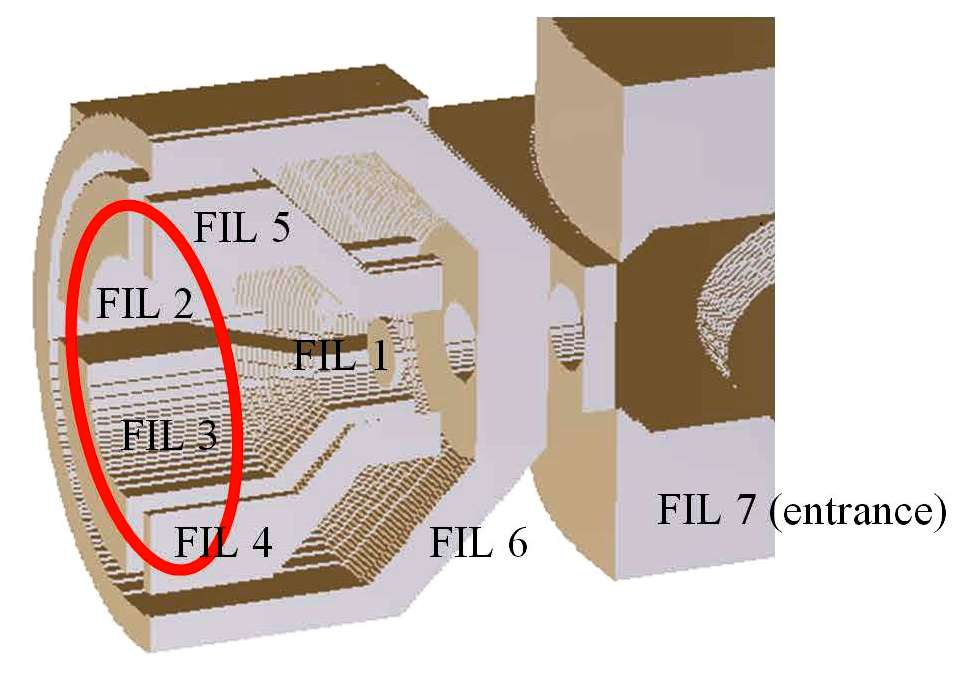
\includegraphics[width =0.85\textwidth]{Setup/Proto_FilEl_sim.jpg}
			\end{subfigure}
			\begin{subfigure}{0.5\textwidth}
				\centering
				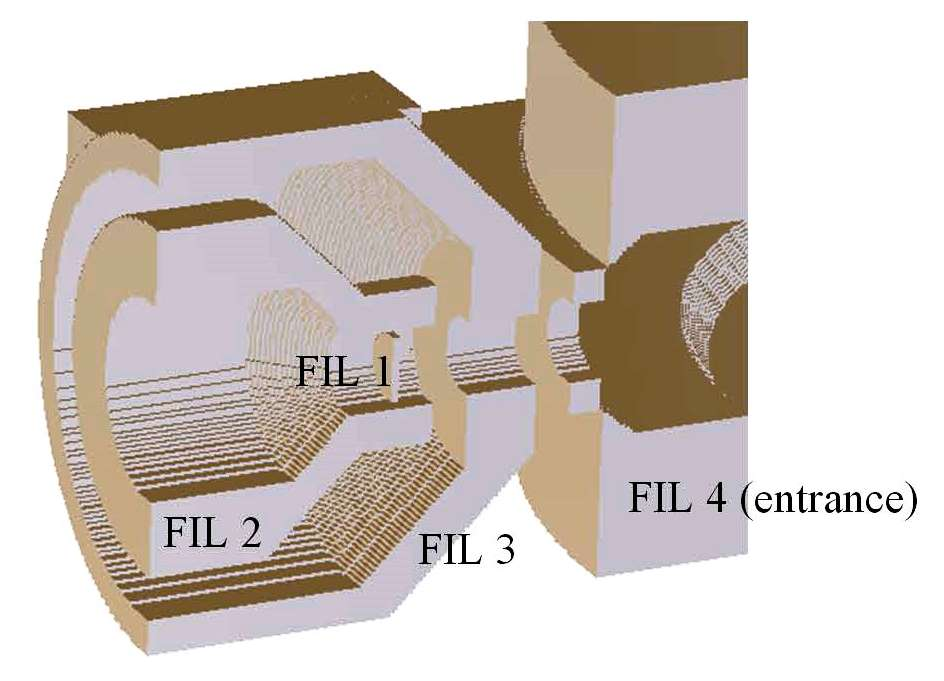
\includegraphics[width = 0.85\textwidth]{Setup/PFM_FilEl_sim.jpg}
			\end{subfigure}
			\caption{Left: Prototype filament housing. Right: PFM filament housing.}
			\label{fig:SetupFilElSim}
		\end{figure}

		\begin{figure}[h]
			\centering
			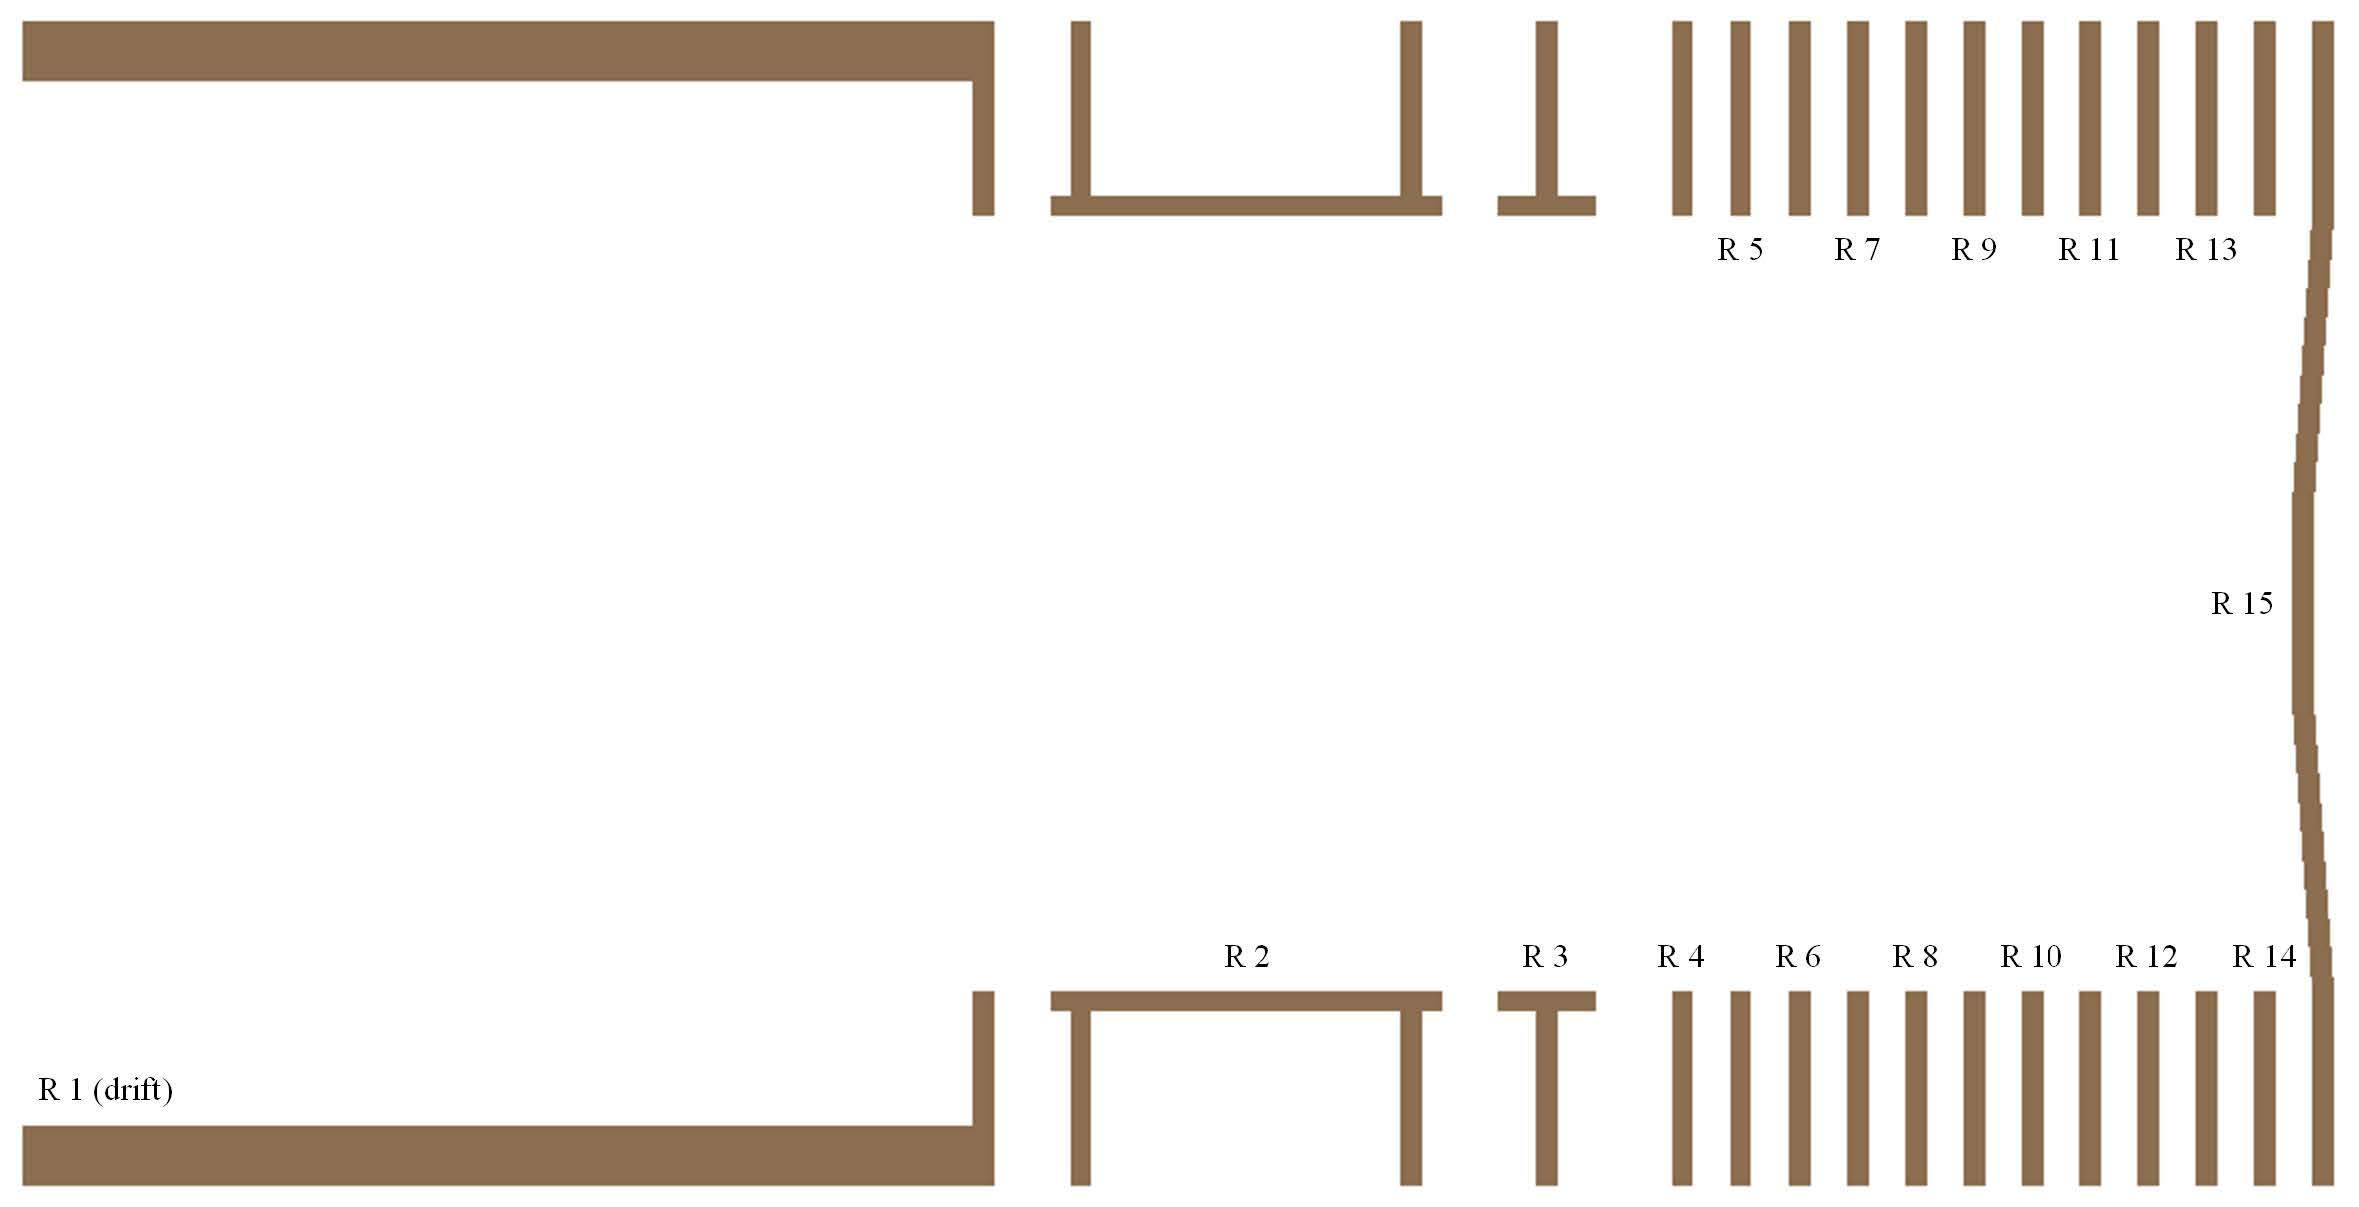
\includegraphics[width=0.9\textwidth]{Setup/Prototype_Reflectron_sim.jpg}
			\caption{SIMION Model of the ion-mirror of the NIM Prototype \cite{Diss_Meyer}.}
			\label{fig:SetupProtoReflSim}
		\end{figure}
		
		\begin{figure}[h]
			\centering
			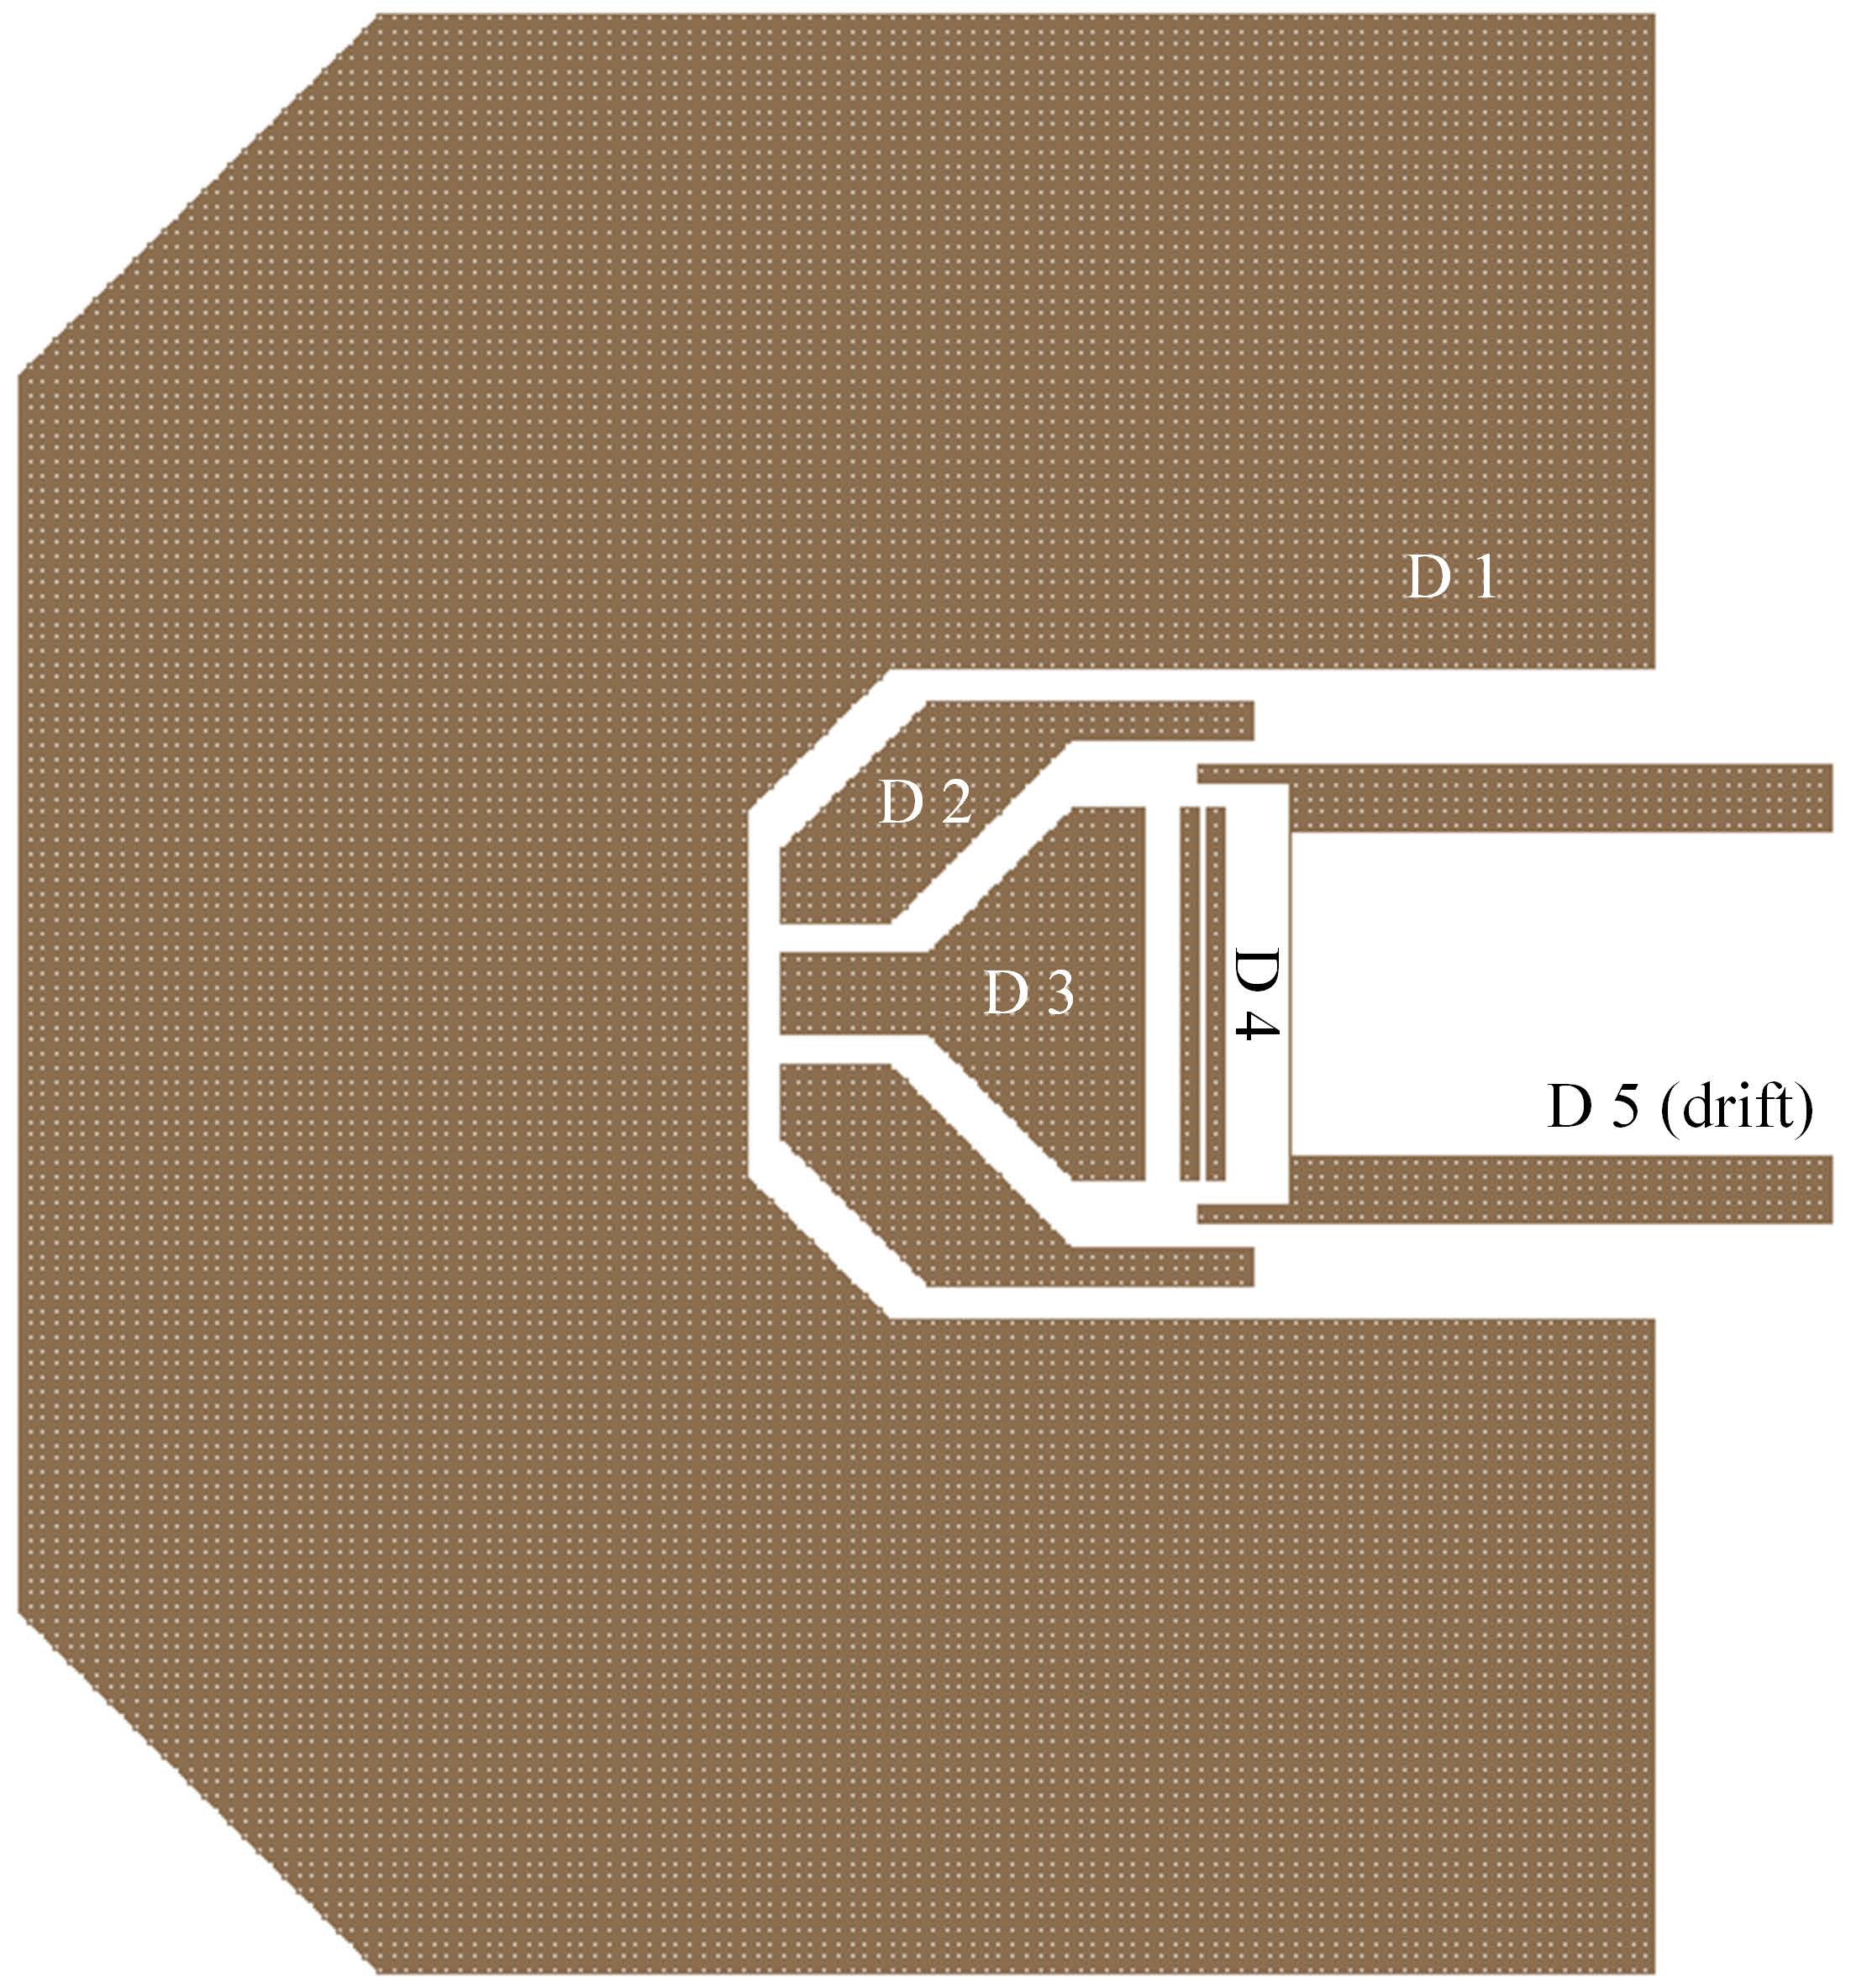
\includegraphics[width=0.4\textwidth]{Setup/Prototype_Detector_sim.jpg}
			\caption{SIMION Model of the detector of the NIM Prototype \cite{Diss_Meyer}.}
			\label{fig:SetupDetSim}
		\end{figure}
		
		\begin{figure}[h] % Exchange reflectron through ion-mirror
			\centering
			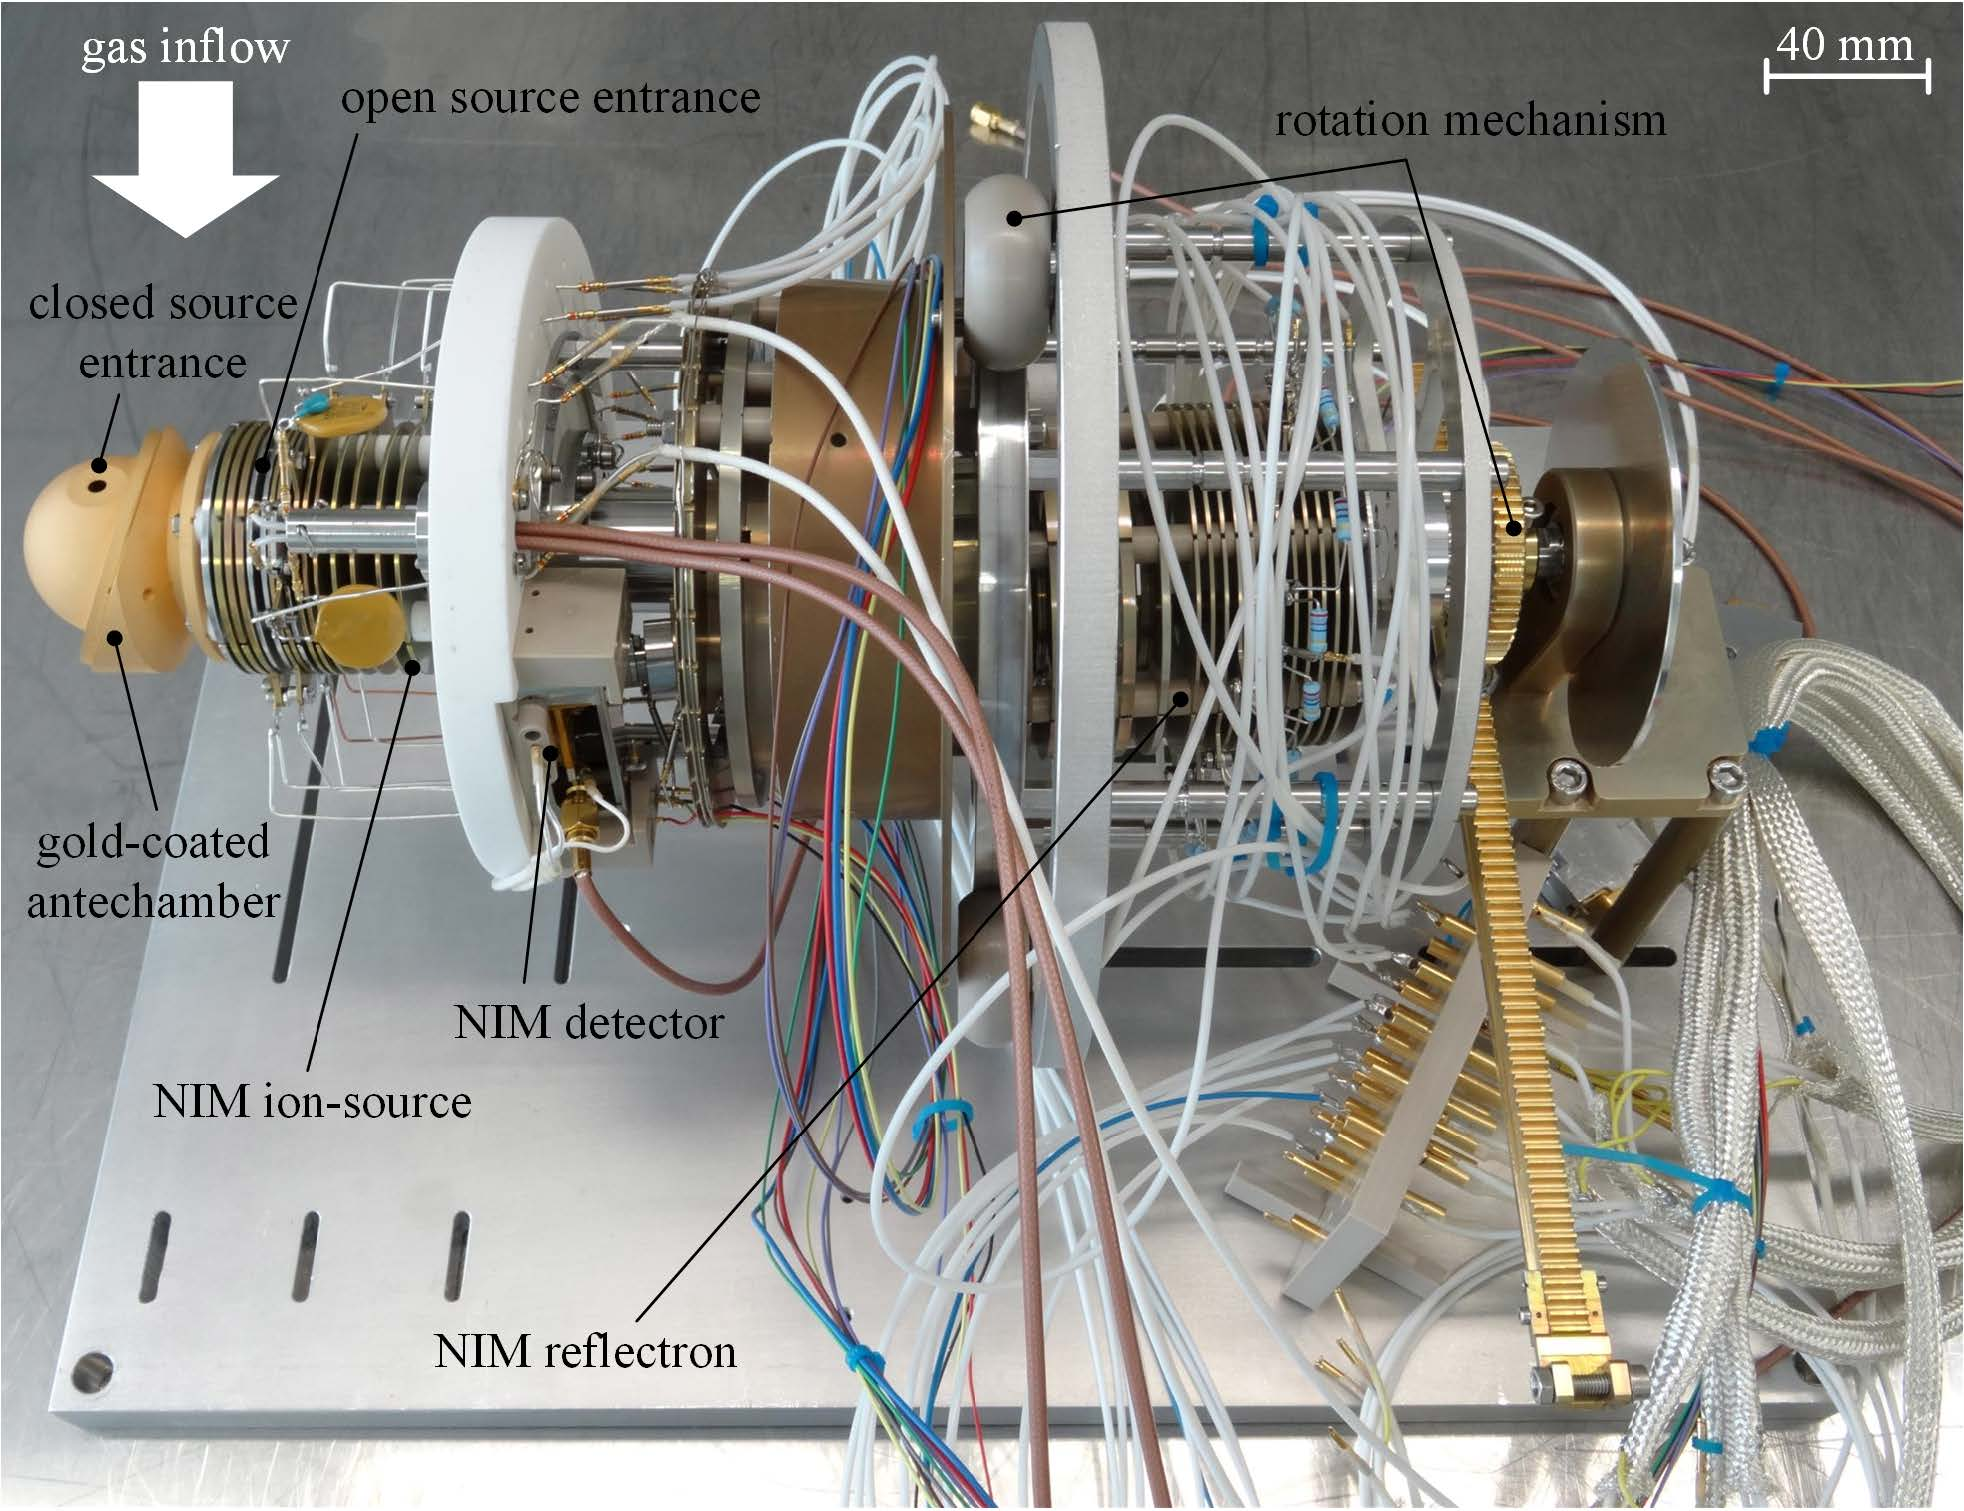
\includegraphics[width=\textwidth]{Setup/Prototype_totPic.jpg}
			\caption{NIM Prototype \cite{Diss_Meyer}.}
			\label{fig:SetupProto}
		\end{figure}
		
		\begin{figure}[h] % Exchange picture through a picture collection (EGU2020 slid of the sensor in different states) Add a picture, where the inner parts are visible for comparison. Include a lineal ruler into the pictures.
			\centering
			\includegraphics[width=0.8\textwidth]{Setup/PFM_in_calib_Setup.JPG}
			\caption{NIM PFM sensor head in calibration setup.}
			\label{fig:SetupPFM}
		\end{figure}
		
		
		\begin{comment}
		
		1x new IS with declaration
		1x comparison of the two where the two sources are overlapped
		Take chapter Prototype and PFM together in one chapter depending on how much there is to write in the Prototype chapter.
		PFM has more details.
		In case of 1 Chapter, don't overlay the pictures, simply show both IS separately and mark the changes in the PFM/ Prototype pictures (IS, Fil). Reflectron make a short not about the changes. Detector stays the same. Antechamber got bigger. Shutter missing in Prototype.
		
		Startconfiguration.
		
		Gleiches Schema wie bei Prototyp (IS) einfügen aber die Änderungen markieren. Ref. Arbeit von Stefan machen, weil dieses Redesign eigentlich noch von seiner Arbeit ist.
		Simulations Schema mit Quelle (für El-Benamslung einfügen. Evt. nur Schema von Quelle einfügen, weil hauptsächlich da die # der Elektroden geändert hat)
		
		Dann Fotos von der Harware zusammensuchen und zusammenstellen.
		
		Referenz auf Rack (am Anfang wurde das Gerät auch mit der Laborelektronik betrieben). Schema mit dem Kabel für die LVs zwischen dem Rack und der Kammer (Fotos). Anschlüsse fotografieren. Liste welche Elektrode wo angeschlossen wird (Liste von Prototyp anpassen)
		
		Show the model of the PFM and then explain the differences between the two models. Refere to the test campaigns of the Prototype, where the different parts were tested.
		
		\end{comment}
		
		\textbf{Ion-Optical System Proto Flight Model}\\ % TBD Dec. 2020
		
		
		% PFM Simulationen Stand. Instrumentenvergleich. Beide Schemas von Quellen übereinander legen für den Vergleich der beiden Quellen am Anfang. Bei den Experimenten die kleinen Anpassungen jeweils bei den Expereimenten einfügen. Subchapter of NIM instrument.
	
	
	\subsection{Test facilities/ Test Tools}\label{subsec:setupTestTools} % Bei test tools wäre das simulationsprogramm auch inbegriffen
	
	% Testanlagen hier beschreiben in einem einzelnen Unterkapitel falls sie weiter ausgeführt werden. Evt. auf CASYMIR nur einen Verweis machen. SATANS etwas genauer auseinander nehmen.
	% Explain the simulation programm as far as it is needed. This chapter will be referenced from the experiments chapter. In experiments, simulations and tests will be compared -> reference on how the simulations work are explained here as far as needed.
	% SATANS
	


%-------------------------------------------------------------------------------------	
	%% STROFIO chamber
	\begin{comment}
		Include here the whole cabling? No. Refer to Diss Stefan for the description of the start electronics. -> show the changes later in Chap. Experiments.
		Picture inside the STROFIO chamber. One picture of the current test setup with the rotation mechanism. Show on a picture where the gas enters the IS and the antechamber.
		Static gas measurement: Measurement with the STROFIO chamber with a set background gas. (Or also describe it in the different experiments? Make also a note there because then it is clear how the different measurements where performed)
		
		If there is not enough txt for a chapter, include it at the description of the NIM prototype.
	\end{comment}
	
	
%---------------------------------------------------------------------------------------
	%% Simulation Prototyp (in the simulationen, the simplification of the ionsource is already implemented)
	\begin{comment}
		7 lenses, no filament (you set the place and flight direction of the entering produced ions -> no filament in the current simulation model)
		
		flight reflectron
		
		Pulser: you can set the most important parameters of the pulse shape in the simulation.
		
		
		
		
		
		
		
		
		
	\end{comment}
	
	
%---------------------------------------------------------------------------------------
	% SATANS. Not mention. No enough time. Did a few tests. Or if it is mentioned, make a reference and make only a brief overview. -> Boris has to investigate this subject a bit further. Give him the results made until then -> adaption of the shape of the discharge pins.
	\begin{comment}
		further steps. Further investigation of the ion source to get more ions.
		
		
		
	\end{comment}
	
	
	
	
